While on-site assertion of an intersection is plausible, the scope of a single observer is limited, as one can only keep track of 
so many cyclists at once. Likewise with analyzing recorded video footage, while not bound by time, is still a time-consuming process, 
especially as the views of cyclists can be obstructed by other passing vehicles or permanent fixtures. 
As an example, previous desire line studies conducted by Copenhagenize were done by keeping counts of hand-written references to trajectories (figure \ref{manual_desire_line}).
\ \\

\raggedbottom
\noindent
\begin{tabular}{@{}cc}
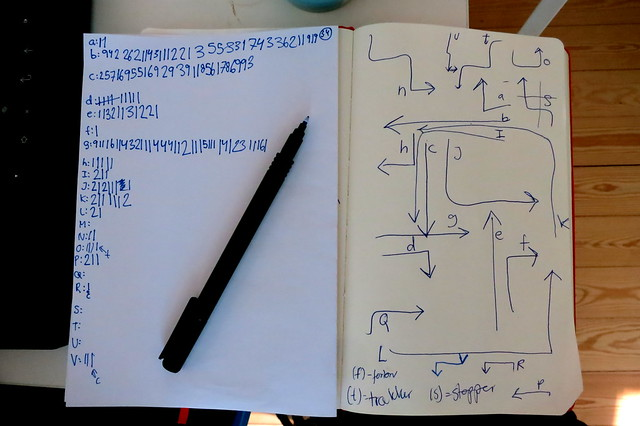
\includegraphics[width=1.0\columnwidth]{desire_line_counts} 
\end{tabular}
\captionof{figure}{Manual desire line counts (Copenhagenize, 2014)}
\label{manual_desire_line}
\

\subsection{Initial tests with OpenDataCam}
As a baseline, we deployed an OpenDataCam setup using pre-recorded footage from the Dybbølsbro intersection in Copenhagen.
Our setup ran on an Nvidia Jetson Xavier NX combined with two Raspberry Pis for filming/streaming video from the intersection.

Our goal was to extract pre-defined desire lines using the counting line functionality. We did this by drawing an initial 
'base line' followed by two (or more) additional counting lines, which would allow us to branch cyclists into multiple segments (figure \ref{base_line}). Inspecting the
overlap of unique cyclists who passed both the base line and one (or more) of the branching lines would yield which path
they took through the intersection. 
\ \\

\ \\
\raggedbottom
\noindent
\begin{tabular}{@{}cc}
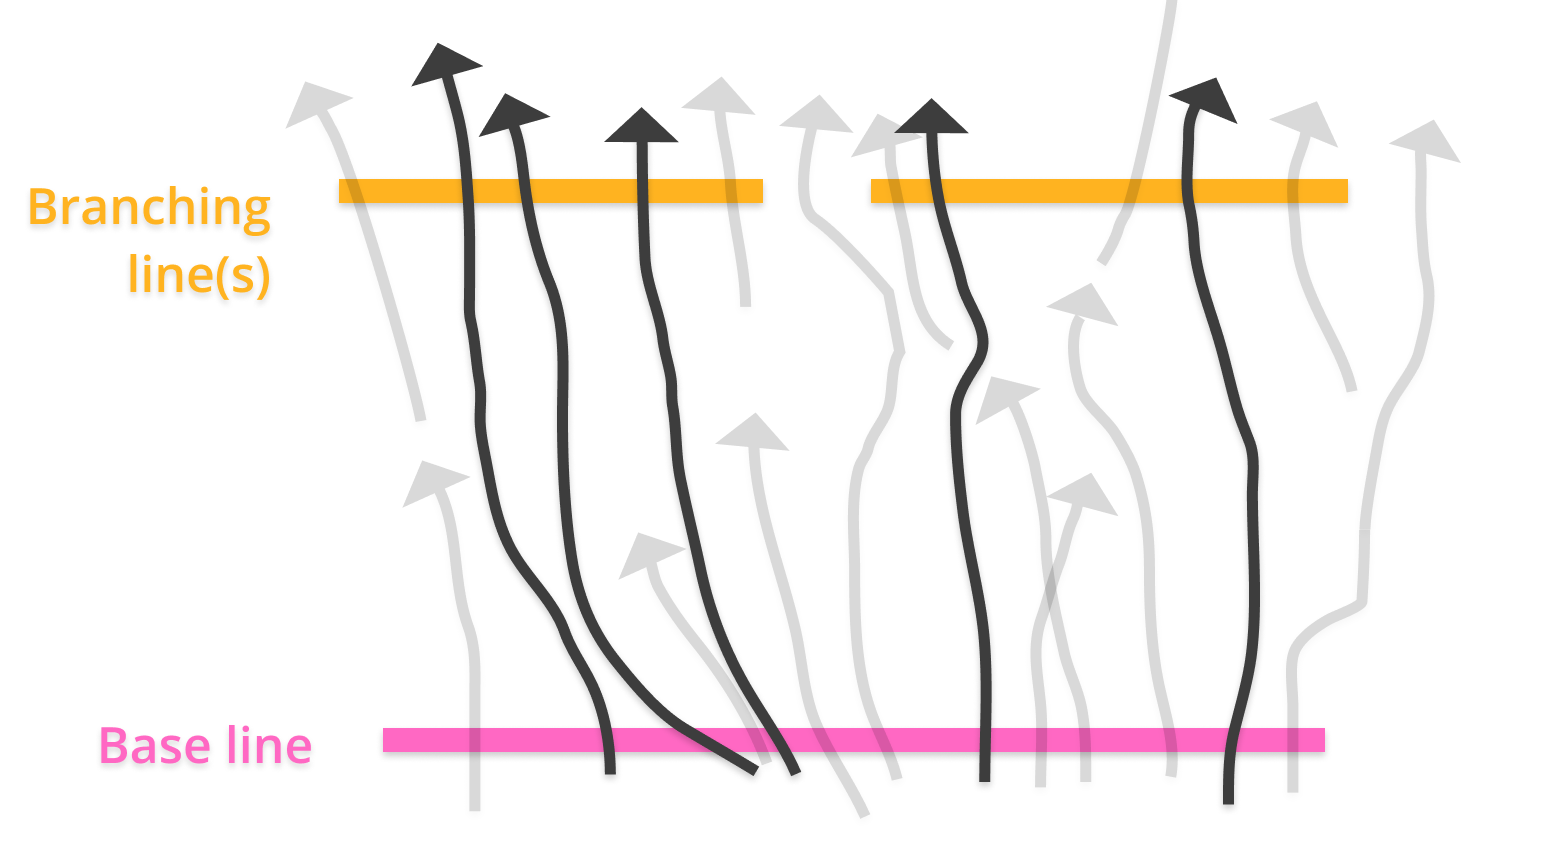
\includegraphics[width=1.0\columnwidth]{base_line} 
\end{tabular}
\captionof{figure}{'base line' (pink) and branching lines (orange)}
\label{base_line}
\

However, this approach was limited by the performance of the detection of cyclists implemented in the current 
version of OpenDataCam (YOLOv4). Due to the intermittent identification of cyclists, the tracking algorithm would constantly 
re-identify the same cyclists as new ones. Thus, even when the same cyclist passed both the 'base line' and one of the 
branching lines, they would not be included in the desire line count.
\ \\
 
We discuss the findings derived from OpenDataCam in our case study in later sections of the report.

\subsection{Proposal}
We wish to improve and extend the functionality of OpenDataCam, centering around cyclists and intersections.
Using a newer version of YOLO for object detection will result in better tracking accuracy for cyclists, 
and thus more complete trajectories.
While OpenDataCam emphasizes real-time metrics on traffic, we specifically work with 'post-processed' footage 
from intersections, and therefore we can apply further assumptions about the tracking behavior to improve accuracy.
\ \\

The aforementioned issue of keeping track of unique cyclists as their view is temporally obstructed is also faced by 
object tracking algorithms in video. In theory, a top-down overhead view overlooking the center of the 
intersection would be optimal for minimizing obstruction.
However, the height required for such a recording setup, as well as the lack of permanent fixtures, makes this 
approach very impractical. 
Current state-of-the-art object detection algorithms (e.g.~YOLO) also perform worse at categorizing objects, 
especially bicycles, using an overhead view compared to a semi-frontal view (\cite{overhead}). 
We, therefore, propose deploying a multi-camera setup overlooking an intersection from multiple sides.
\ \\

A top-level aerial view can help identify rule compliance through the intersection by comparing
the shares of cyclists using chosen desire lines to reach the same destination. 
To bring nuance to the analysis, one can dig into the footage to assess the behavior of 
each identified cyclist using a specific desire line. 
This can provide insights about the context to non-intended behavior such as state of traffic signals, 
vehicles and the momentum of other cyclists.